\documentclass{instructions}

\usepackage{xspace}

\newcommand{\git}{\texttt{git}\xspace}
\newcommand\bs{\char`\\}

\graphicspath{{figs/}}

\title{Practical 3: Incremental Encoder}
\date{\today}

\summary{
    This week, you will build and fit to your DC motor an optical incremental
    encoder. Plug it to an Arduino and measure the angular velocity of your
    motor.
}

\objectives{
At the end of the practical, you should:

\begin{itemize}
    \item have build a basic yet accurate incremental encoder
    \item have fit the encoder on your motor shaft
    \item have connected it to an Arduino board and programed the Arduino to read the
        angular velocity of your motor.
\end{itemize}
}

\challenges{

    \begin{itemize}
        \item There's a lot to do! Be quick!
    \end{itemize}
}

\begin{document}

\maketitle


\note{
In your lab journal, \textbf{describe the basic design of each component},
\textbf{how it was constructed} and \textbf{how it was tested}. Add
\textbf{pictures} and link to \textbf{videos} as needed.

Describe as well \textbf{the overall system} and how it performs.

\vspace{1em}

And do not forget: \textbf{write your lab journal as a text file using the Markdown
syntax} and \textbf{push your journal and the pictures on GitHub}.

}

%%%%%%%%%%%%%%%%%%%%%%%%%%%%%%%%%%%%%%%%%%%%%%%%%%%%%%%%%%%%%%%%%%
%%%%%%%%%%%%%%%%%%%%%%%%%%%%%%%%%%%%%%%%%%%%%%%%%%%%%%%%%%%%%%%%%%
%%%%%%%%%%%%%%%%%%%%%%%%%%%%%%%%%%%%%%%%%%%%%%%%%%%%%%%%%%%%%%%%%%


\part{Introduction}

\section{Principle of operation}

This assignment consists of using an LED light source and phototransistor
detector.  When a slotted disc is placed between the light source and detector
and rotated, the circuit will detect each time light can pass from the LED to
the phototransistor, as shown in Figure~\ref{Principle}. Using an Arduino to
count  these  pulses, it  is  possible  to  estimate  the  rotational position
and angular velocity of the disc. 


\begin{figure}[h!]
    \centering
    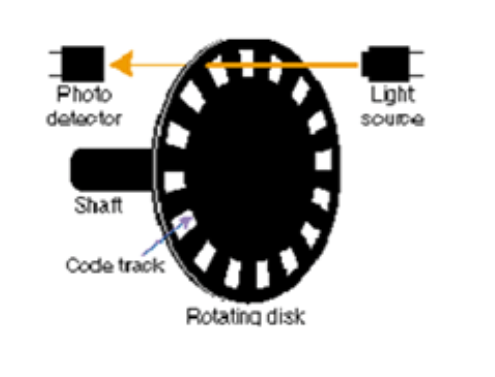
\includegraphics[width=0.5\linewidth]{encoder-000}
    \caption{Basic  operation  of  the  simple  optical  incremental  encoder.  A  light 
source shines light through holes in a disc, which can be detected by a photo 
detector. As the disc rotates, this gives rise to one pulse per hole.}
    \label{Principle}
\end{figure}


\step{Circuit diagram}

The circuit is very simple and shown in Figure~\ref{circuit}. We use an IR LED
as a light source and an IR sensitive transistor to detect its light. They
should be aligned to the LED shines onto the phototransistor, as illustrated in
Figure~\ref{veroboard}. 

\important{Set the power supply to 5V! By doing so, you will not destroy the
semiconductors  if  you  accidentally  connect  it  up  the
circuit  with  the wrong  supply  voltage  polarity.}

\begin{figure}
    \centering
    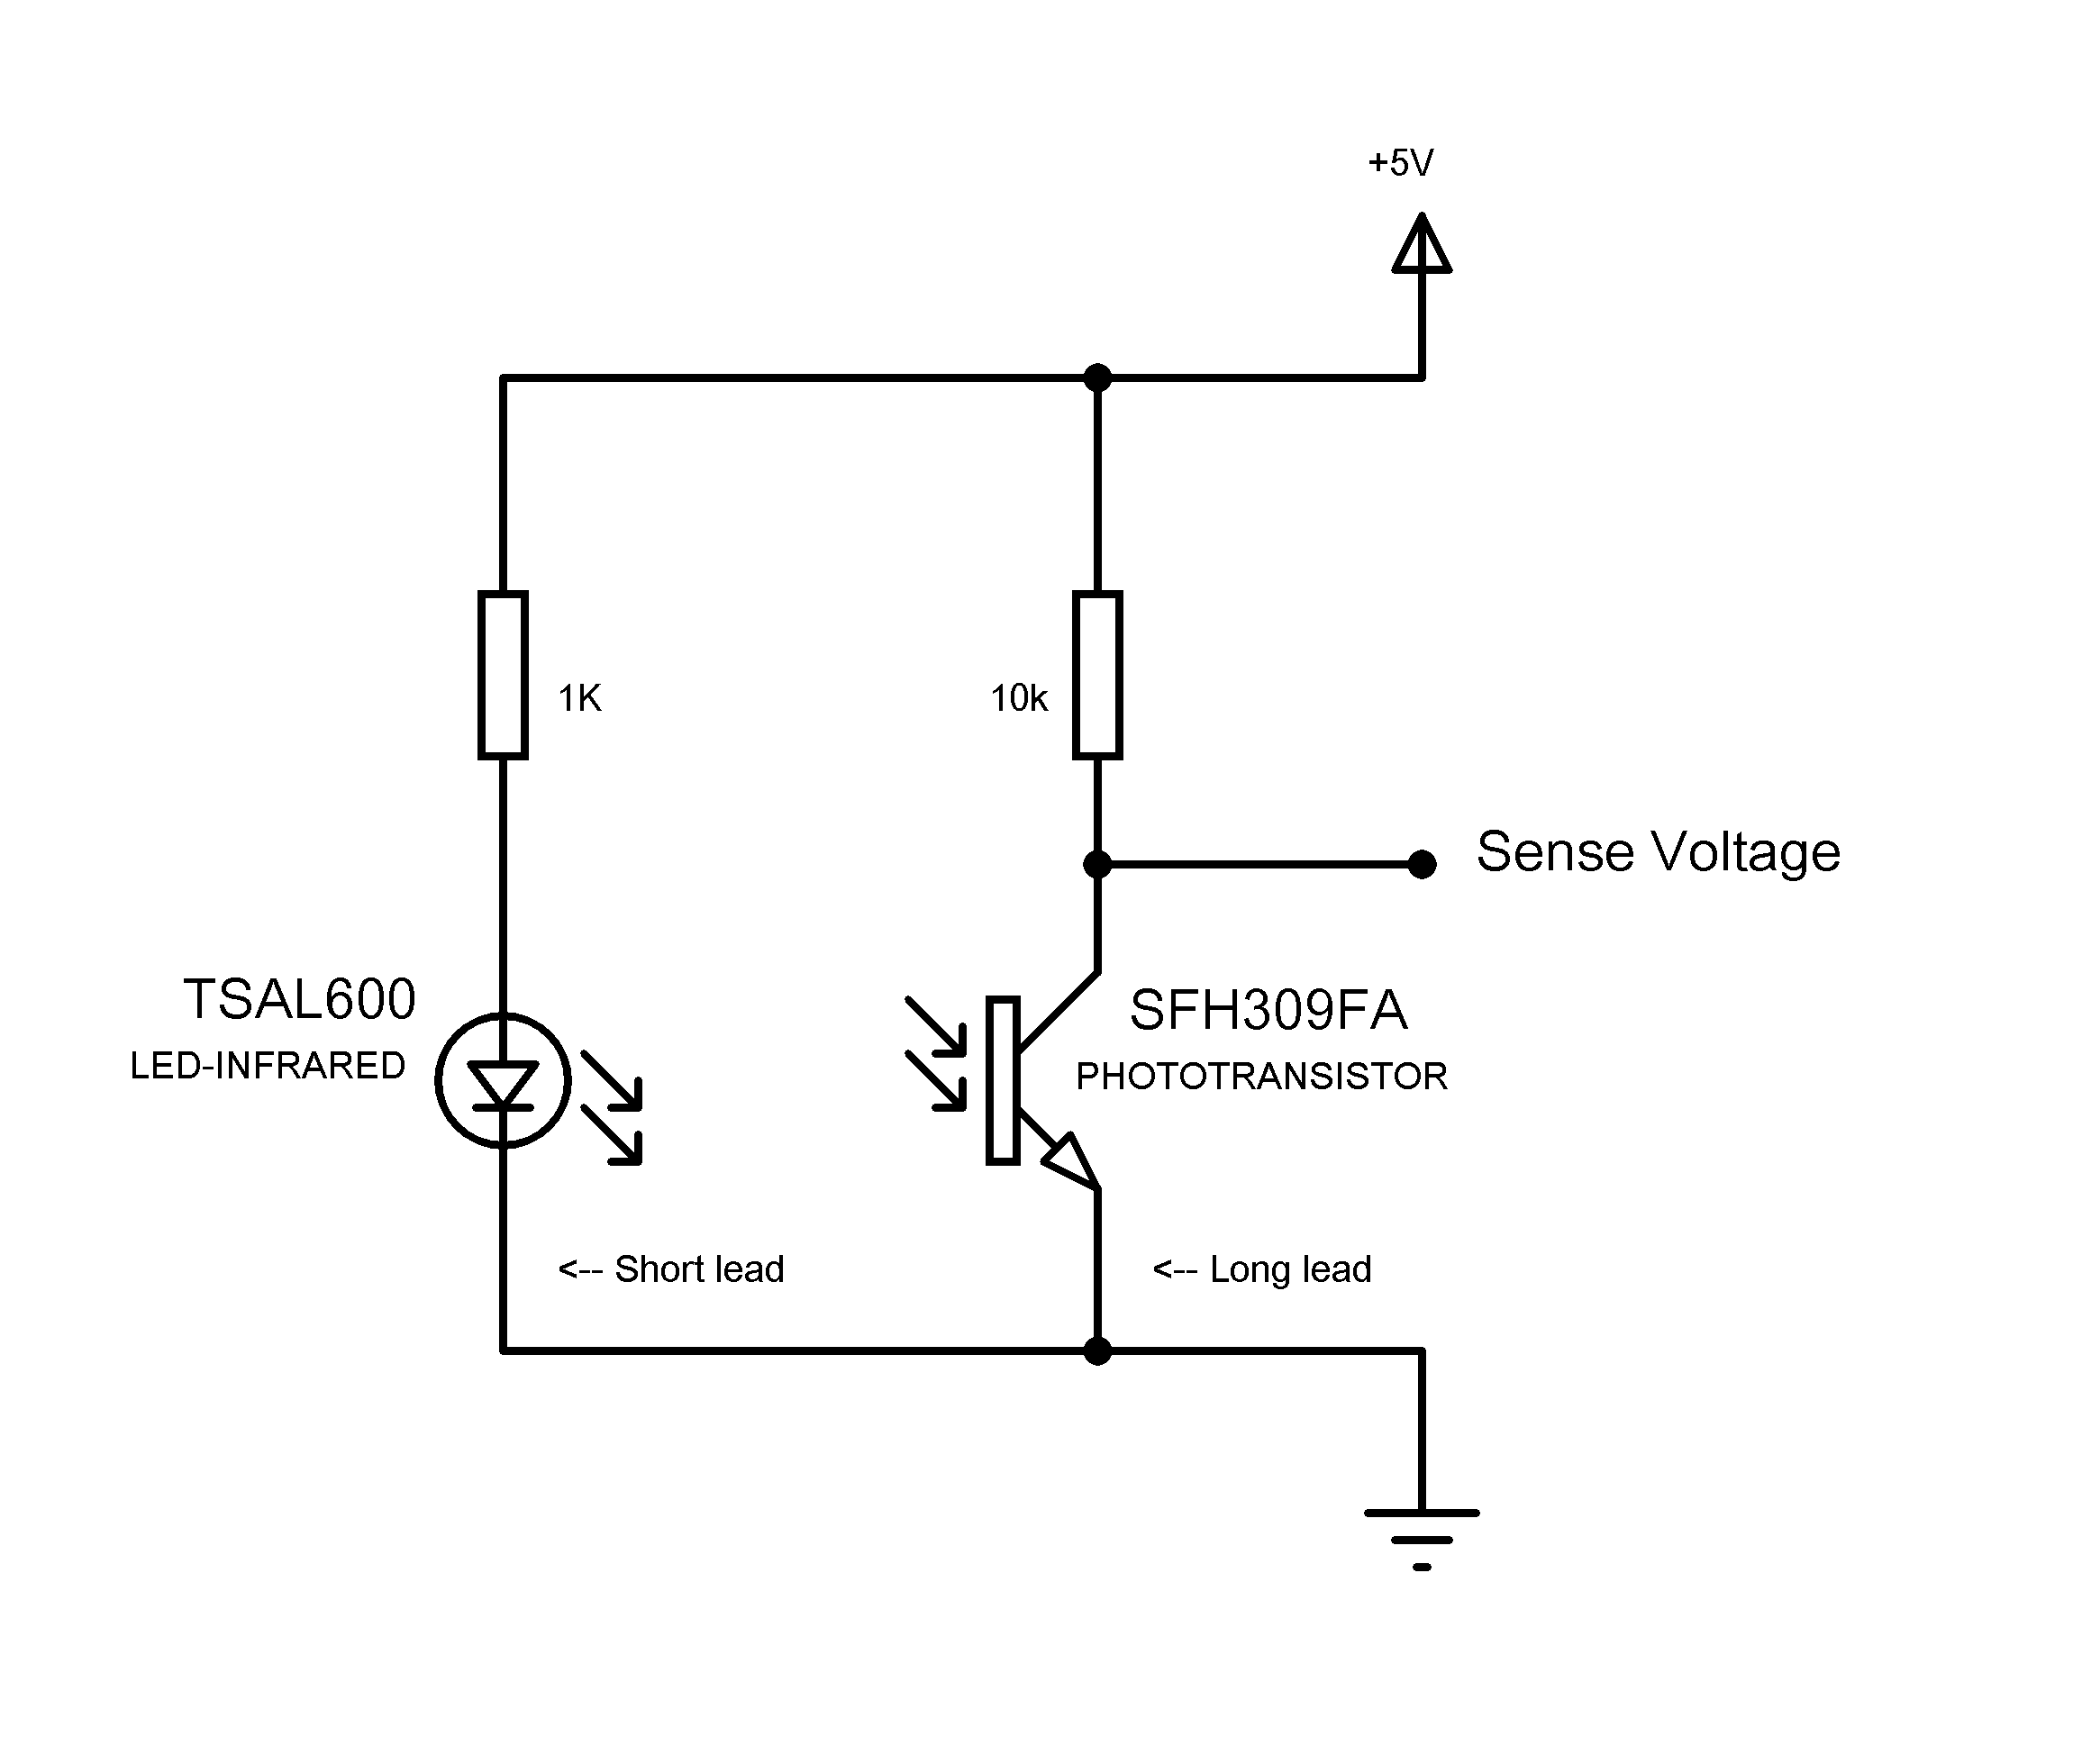
\includegraphics[width=0.7\linewidth]{encoder-001}
    \caption{Simple  IE  circuit.  The  IR  LED  provides  a  light  source  and
    a phototransistor  detects  it.  When  the  light  is  blocked,  the
    phototransistor switches off.}
    \label{circuit}
\end{figure}

You  will  be  provided  will  all  the  necessary  electronic  components: an
IR LED, a IR photo transistor, 1K and 10KOhms resistors, connecting wire and a
piece of Vero board to solder them onto. You need to use a bench power supply to
run the circuit. You will need to use an oscilloscope to check it is working.
Figures~\ref{veroboard} and~\ref{motor-encoder} provide details of these
components. 

\note{If needed, use the resistor colour codes provided at the end of the
instruction sheet to check your resistors' values.}

Build the circuit in stages and test each stage before you progress to the next
stage. 

\step{Build the IR LED light source}

Set  the  power  supply  to  5V.  Connect the red  and  black  wires  to  the Vero
board to supply the circuit with power. Use a 1KOhm resistor to drive the IR
LED from the 5V supply. Note the output light from the IR LED is invisible to
the human eye, although some digital cameras can detect it. 

\step{Build the light detector}

Use a 10KOhms resistor to drive the phototransistor from the 5V supply. Measure
the voltage  across  the  phototransistor. When it receives IR light from
the  IR  LED,  the phototransistor turns on and it should drop only a small
voltage across the emitter and  collector.  When  the  light  path  is  blocked,
the  transistor  will  turn  off  and  the voltage  across  the  emitter  and
collector  will  rise  to  almost  the  supply  voltage.  By monitoring this
voltage it is possible to detect when the light path is blocked. Block the light
with a piece of card and check that it is working. 

\begin{figure}
    \centering
    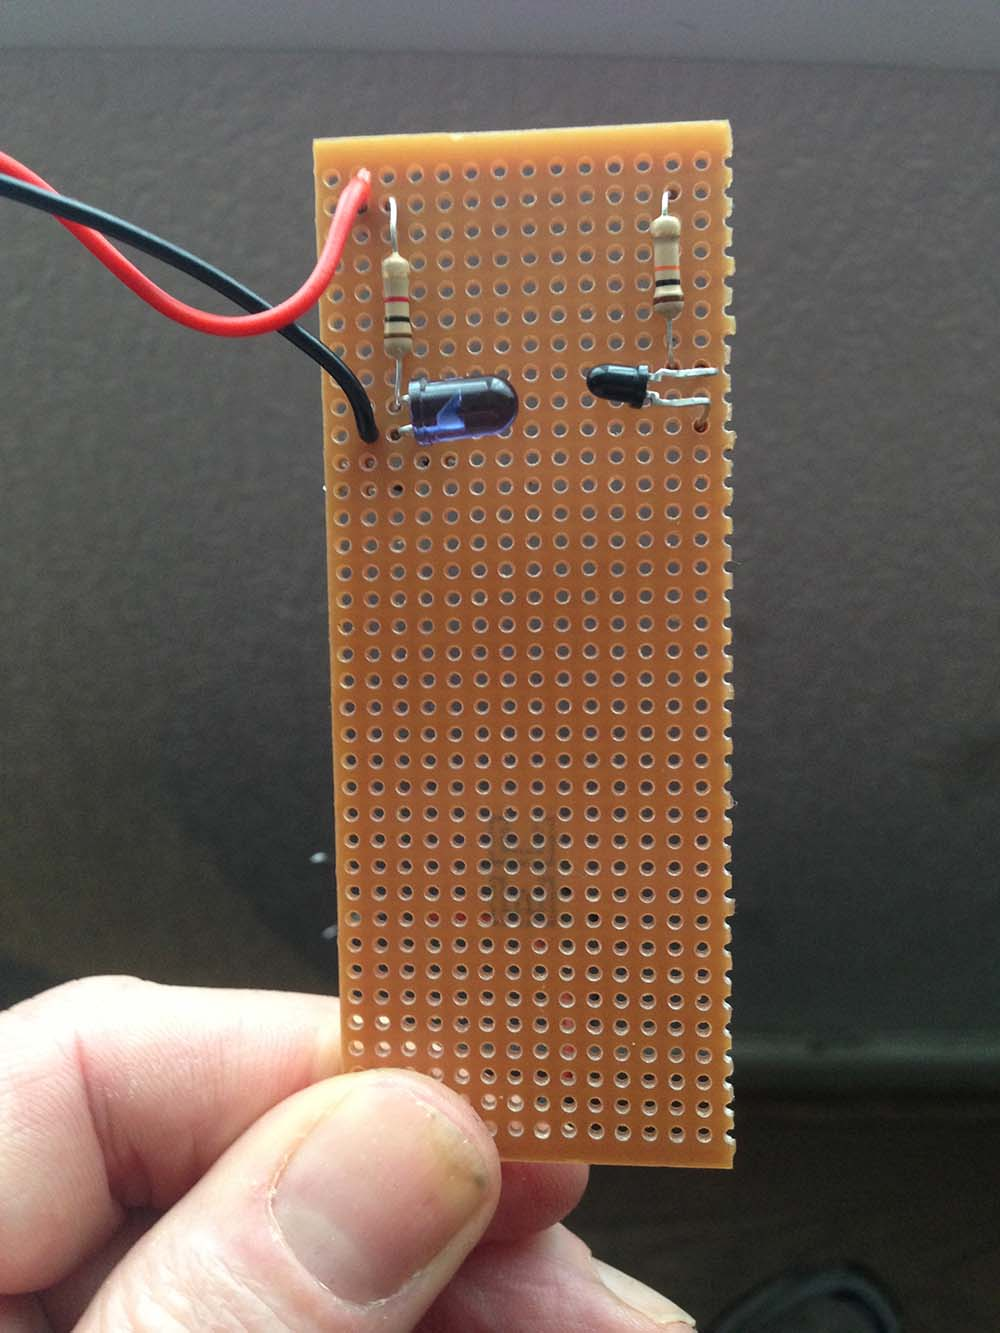
\includegraphics[width=0.6\linewidth]{encoder-006}
    \caption{Finished  Veroboard  circuit.  Make  sure that the LED and the
    phototransistor point towards each other and are far enough off the board
    that you  can  measure  the  rotational  speed  of  the  rotating  disc
    attached  to  the motor in Figure~\ref{motor-encoder}!}
    \label{veroboard}
\end{figure}


\step{Place an encoder disc on the motor}

Cut out a cardboard disc and make a hole in the centre so it fits onto your motor
shaft.  Attach it with blue tack. Cut a sector so that the disc will allow the
passage of light once per revolution (see Figure~\ref{motor-encoder}). 

Hold the disc between the IR LED and phototransistor while it is rotating. You
need to  work  in  pairs  to  do  this.  When  light  is  blocked  by  the
passage  a  disc  rotated  a motor, an oscilloscope can be used to determine the
speed of rotation of motor. How can this be achieved? Run the motor and estimate
its speed of rotation in RPM. 

\begin{figure}[h!]
    \centering
    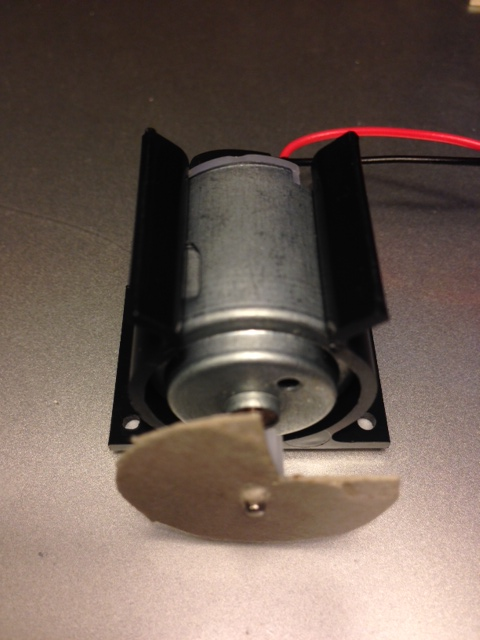
\includegraphics[width=0.5\linewidth]{encoder-007}
    \caption{Cardboard disc attached to motor to break light beam from LED to
    phototransistor. You may need blue tack to attach the disc. Be careful not
    to cut  too  much  away  to  make  the  sector  to  let  light  pass  or  it
    will  no  longer attach to the motor spindle!}

    \label{motor-encoder}
\end{figure}

\note{Do not forget to make \textbf{photos \& videos of your system} for your journal!}

\part{Arduino}

\step{Launch the Arduino IDE}

Open the Arduino IDE, plug the provided Arduino, and make sure the IDE is
correctly configured for your card (check the card type -- Arduino UNO -- and
the port -- likely \texttt{/dev/ttyACM0}).

\begin{center}
    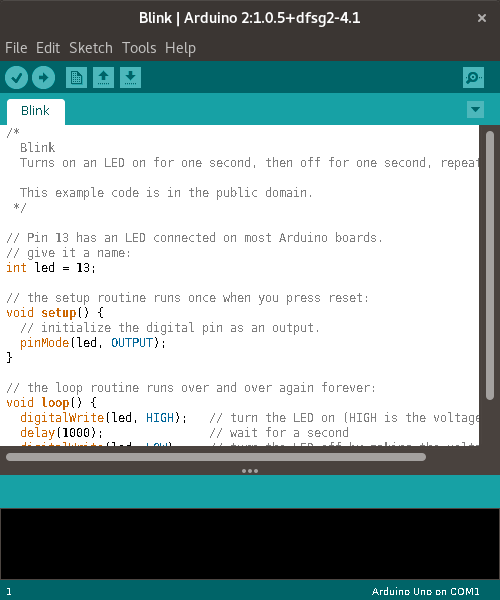
\includegraphics[width=0.5\linewidth]{arduino-ide}
\end{center}

\step{Connect your encoder}

Use the following diagram to connect your encoder to the Arduino.

\begin{center}
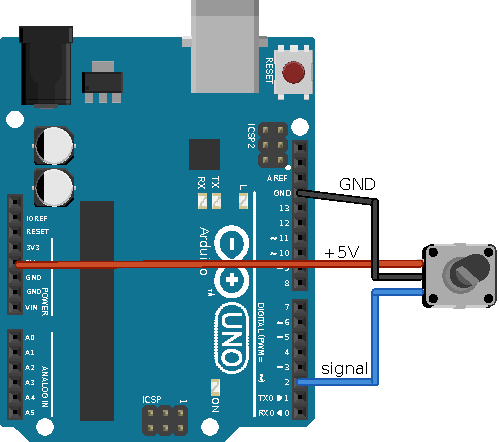
\includegraphics[width=0.6\linewidth]{arduino-encoder}
\end{center}

Using the following program, test whether your encoder is correctly connected. Manually block the light path of your light detector: it should cause the Arduino LED to blink.

\begin{cppcode}
const byte ledPin = 13;
const byte interruptPin = 2;
volatile byte state = LOW;

void setup() {
  pinMode(ledPin, OUTPUT);
  pinMode(interruptPin, INPUT);

  // configure the interrupt call-back: blink is called everytime the pin 
  // goes from low to high.
  attachInterrupt(digitalPinToInterrupt(interruptPin), blink, RISING);
}

void loop() {
  digitalWrite(ledPin, state);
}

void blink() {
  state = !state;
}
\end{cppcode}



\step{Calculate the angular velocity of your motor}

Modify the program to count the number of pulses. Use this count to output on
the serial port the speed of your motor every second.

The following code example shows how to write to the serial port every second:

\begin{cppcode}
void setup()
{
  Serial.begin(9600);           // set up Serial library at 9600 bps
}

void loop()
{
  Serial.println("Hello world!");  // prints hello with ending line break 
  delay(1000);                     // wait 1s
}
\end{cppcode}

\more{Check on the web the other \emph{modes} of \cpp{attachInterrupt}. A wise
choice and a bit of math should let you improve the resolution of your encoder.}

\part{Components}

\begin{figure}[h!]
    \centering
    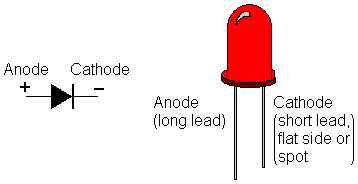
\includegraphics[width=0.4\linewidth]{encoder-008}\\
    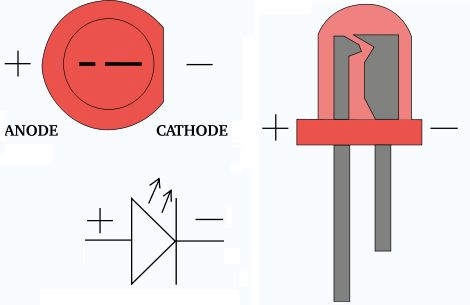
\includegraphics[width=0.4\linewidth]{encoder-010}
    \caption{Led pins – same for IR LED }
    \label{}
\end{figure}


\begin{figure}[h!]
    \centering
    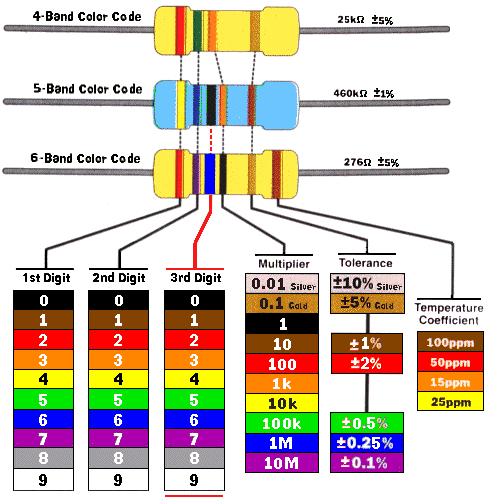
\includegraphics[width=0.6\linewidth]{encoder-012}
    \caption{Resistor colour codes}
    \label{}
\end{figure}
 

\begin{figure}[h!]
    \centering
    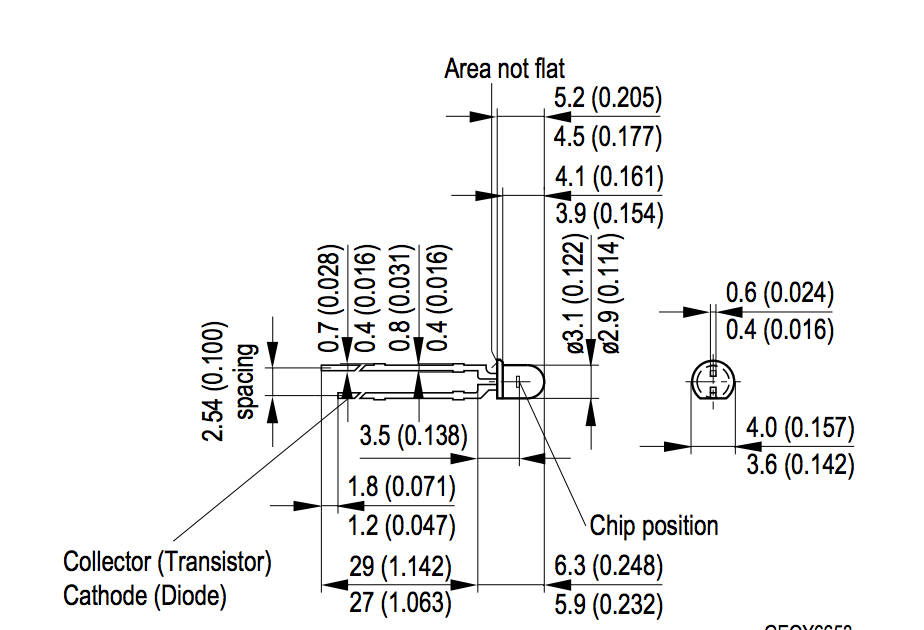
\includegraphics[width=0.9\linewidth]{encoder-013}
    \caption{SFH309FA connection polarity}
    \label{}
\end{figure}
 

\end{document}
